\section{Mathematical Model of the PlayStation Controller}
To come up with a theoretical analysis of the transfer function, a simplified mechanical schematic has been drawn. This schematic can be seen in figure \ref{fig:mechanical_schematic}.
\begin{figure}[h!]
	\centering
	\includegraphics[width=0.6\linewidth]{Figs/mechanical_schematic}
	\caption{Simplified mechanical schematic of the actuation system with the stimulator.}
	\label{fig:mechanical_schematic}
\end{figure}

The equations of motion can be formulated with the major parameters defined in the schematic. A full explanation of all parameters can be seen in table \ref{tab:setup_params}. The variables with subscript $1$ refer to the first mass element, the carriage in its guideway, whereas variables with subscript $2$ refer to the stimulator, also known as the palm pad. For the motor the subscript $m$ has been used.
	
\begin{figure}[h!]
	\centering
	\begin{tabular}{|l|c|c|}%designator | explanation | unit
		\hline
		 Designator & Explanation & Unit \\ \hline \hline
		$T_m$ & Motor torque & [Nm]\\ 
		$T$ & Output torque acting on carriage& [Nm]\\
		$\theta_m$ & Motor angle & [rad]\\
		$\theta$ & Clamp link angle & [rad]\\  
		$L_{CL}$ & Clamp link length & [m]\\
		$m_{1}$ & Mass of the carriage in its guideway & [kg]\\
		$m_{2}$ & Mass of the stimulator & [kg]\\
		$x_{1}$ & Position of the carriage in its guideway [m]\\
		$x_{2}$ & Position of the stimulator & [m]\\
		$k_{eq}$ & Equivalent spring constant & [N/m]\\		$b_{sp}$ & Spring damping coefficient & [Ns/m]\\
		$n$ & Reduction gear ratio & [-]\\
		$k_{op}$ & Spring constant of the operator & [N/m]\\
		$b_{op}$ & Damping coefficient of the operator & [s/m]\\
		$J_T$ & Total inertia of mechanical setup & [$\textit{kgm}^2$]\\
		\hline
	\end{tabular}
	\caption{Setup parameters}
	\label{tab:setup_params}
\end{figure}
	
\subsection{Assumptions}
First of all, it is important to mention that the transfer function is non-linear, due to the motor angle $\theta_m$ that determines the force acting on the carriage with mass $m_1$. As an initial approach however, this effect has been neglected. More specifically, it is assumed that $\theta \ll 1$ and $\cos{(\theta)} \frac{T_m}{L_{CL} } = F_{carr} $ becomes $\frac{T_m}{L_{CL} } \simeq F_{carr} $. Here the angle $\theta$ is the angle of the lever, pushing the carriage (ie. $\theta_m = n \theta$). \\
Furthermore, there are several types of friction in the system: the intrinsic friction within the motor and its reduction gear, inside the bearings and the carriage in its guideway. Additionally the springs have a non-negligible damping coefficient. In this work the overall friction and the spring damping have been merged and are represented by the friction coefficient $b_{sp}$. The stimulator, is not in contact with the controller, but with the operator. To model the damping of the skin of the operator and the friction between the skin and the palm pad, the damping coefficient $b_{op}$ has been introduced. Similarly the spring constant of the operator's skin is modeled by $k_{op}$.\\
	
\subsection{Spring Constant and Damping Coefficient of the Operator's Hands}
The order of magnitude of the two coefficients $k_{op}$ and $b_{op}$ are discussed in \cite{Kuchenbecker2003} \cite{Park2014} \cite{Speich2005}. They all indicate parameters varying in the same order of magnitude, namely $k_{op} \simeq 400$N/m and $b_{op} \simeq 5$Ns/m.\\
	
\subsection{Identification of the Spring Damping Coefficient}
The damping coefficient of the spring $b_{sp}$ can be found by comparing the theoretical results of the frequency response analysis with the experimental findings. In fact, for the experimental setup, the stimulator has been fully blocked and therefore the operator's spring coefficient can be seen as infinitely stiff.\\
By varying $b_{sp}$ and Bode-plotting the results of the analytical transfer function, the coefficient's order of magnitude can be found. In order to do so, the analytical transfer function has to be identified.
	
\subsection{Expected Transfer Functions}
The system can be cut into two major transfer functions. The block diagram including these two transfer functions is depicted in figure \ref{fig:2tf_block_diagram}. 
	
\begin{figure}[h!]
	\centering
	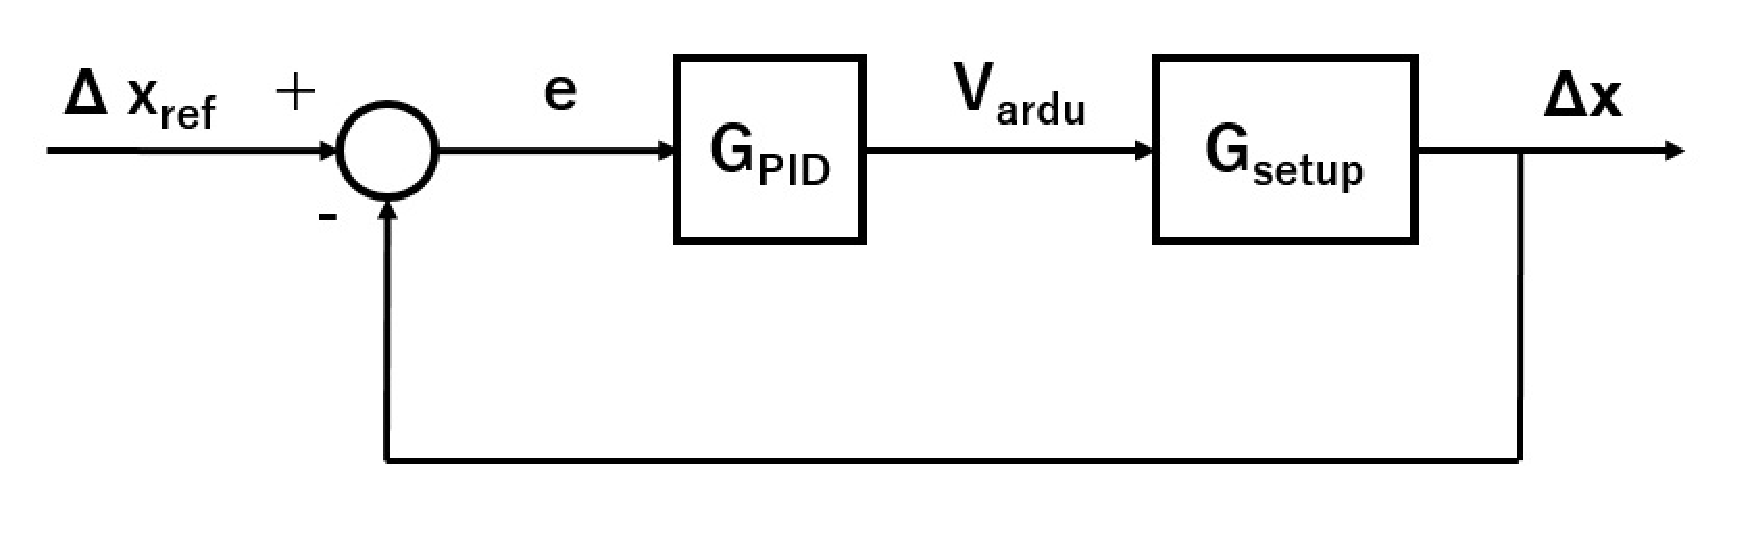
\includegraphics[width=0.6\linewidth]{Figs/2tf_block_diagram}
	\caption{Block diagram with two different transfer functions.}
	\label{fig:2tf_block_diagram}
\end{figure}

According to this figure one can obtain a transfer function of the following form:

\begin{equation}
	F(s) = G_{PID}(s)G_{setup}(s) = \frac{V_{ardu}}{E}\frac{\Delta X}{V_{ardu}} = \frac{\Delta X(s)}{E(s)}
	\label{eq:complete_tf}
\end{equation}
where $V_{ardu}$ is the voltage output of the Arduino for controlling the motors. Using this form one can calculate the individual transfer functions and finally relate the compression of the springs $\Delta x$ to the compression given as reference $\Delta x_{ref}$, since $\Delta X_{ref} / \Delta x = F/(1+F)$.
	
\subsubsection{PID Transfer Function}
The transfer function given by the PID-controller is very straight-forward and can be taken out of any control theory book \cite{Dutton1997}. 
Since the Arduino has limited resolution with floating point operations, the error and reference have been converted into micrometers. To keep the gains consistent between the Arduino code and the matlab script for analytical analysis, the multiplication factor $K_{\mu m}$ to get from the reference distance in meters to micrometers has been introduced. Furthermore, an offset has been added ($K_{bit-offset} = 128$) to allow for negative armature voltages and lastly the PID value has been converted to the Arduino output voltage, where $255$ corresponds to $5$ V. The transfer function is given in equation \ref{eq:tf_pid}. 
\begin{equation}
	G_{PID} (s) = \frac{V_{ardu}(s)}{E(s)} = (K_{\mu m} (K_P + \frac{K_I}{s} + K_Ds) +K_{bit-offset}) K_{PID2Vardu}
	\label{eq:tf_pid}
\end{equation}

Finally, there is also the gain of the amplifier in voltage mode, which converts the voltage of the Arduino into the voltage applied to the motors. This gain is $K_{ampl} = 10$Volt/Volt. To this voltage an offset voltage of $V_{offset} = -25$V is added.\\
	
\subsubsection{Motor Equations}
The second transfer function relates the motor torque $T_m$ to the Arduino voltage as well as the output $\Delta x$ to $T_m$. Due to the back electromotive force these two parts are related and have to be treated as a whole.
	
The output torque $T_m$ of the motor can be calculated using the sum of all torques and the conversion parameters intrinsic to the motor.\\
Similar to the setup and analysis in \cite{Junior2016} the equations of the motor are given as:
\begin{equation}
	L_a \frac{di_a}{dt} + R_a i_a + K_{emf} \dot{\theta }_m = V_a
\end{equation}
where $L_a$ is the armature inductance, $R_a$ the armature resistance and $i_a$ the armature current of the motor. $K_{emf}$ is the back electromotive force constant also given by the motor. $V_a$ is the armature voltage and $\theta_m$ is the angle of the motor shaft.\\
Furthermore, with Newton's law, the sum of all torques must be zero, or:
\begin{equation}
	J_{T} \ddot{\theta }_m - \frac{k_{eq} L_{CL}}{n} \Delta x - \frac{b_{sp} L_{CL}}{n} (\dot{x}_2 - \dot{x}_1)  = T_m = K_{\tau} i_a
	\label{eq:torques}
\end{equation}
In equation \ref{eq:torques} the parameter $J_{T}$ stands for the total equivalent inertia of the motor, the clamping link and the carriage of mass $m_1$.  $K_{\tau}$ is the proportional current torque gain constant. The moment of inertia can either be calculated as the sum of all inertias seen by the motor shaft, or measured in a simple test.\\ 
	
\subsection{Analytical Inertia Identification}
The total inertia of the system is determined by the inertia of the rotor and gears $J_m$, the inertia of the clamp link $J_{CL}$ as well as the inertia of the carriage assembly with mass $m_1$. The last one can be found by simplifying the load to a point mass at distance of the clamp link's length $L_{CL}$, which yields a moment of inertia of $J_{carr} = m_1 L_{CL}^2$.
The gear box affects the inertia seen by the motor shaft by the square of its ratio $n$:
\begin{equation}
	J_{reflected} = \frac{ J_{load}}{n^2}
\end{equation}

We therefore have a total inertia of:
\begin{equation}
	J_T = J_m + \frac{J_{CL}}{n^2} + \frac{ m_1 L_{CL}^2}{n^2}
\end{equation}
where $J_{CL}$ can be calculated by approximating it as a cantilever with an off-center axis of distance $L_{CL} /2$ \footnote{(2018, June 19th) retrieved from \url{http://www.orientalmotor.com/technology/motor-sizing-calculations.html}}: 
	
\begin{equation}
	J_{CL} = \frac{1}{12}m_{CL}(A^2 + B^2 + 12l^2)
\end{equation}
where $A$ and $B$ are the width and length respectively.\\
The calculated total moment of inertia for the motor with a reduction ration of $n = 112$ is 
$$J_T = 6.87 \times 10^{-8} \textit{ kgm}^2$$.
	
\subsection{Experimental Inertia Identification}
Alternatively, one can approximate the total moment of inertia by applying a constant current on the motor and measuring the acceleration. In this case the traveled distance has been derivated twice to find the acceleration, which results in an amplification of errors. Furthermore, the constant current has been kept very low, (between $20$ and $100$ mA), which led to a slow movement and therefore higher friction impact on the measurements. However, the results are consistent with the theoretically calculated values:
$$ J_T = \frac{7.5 \times 10^{-4}}{n^2} = 5.98 \times 10^{-8} \textit{ kgm}^2$$ 
	
\subsection{Relating $\Delta X$ to $\theta$}
The conversion between the angle $\theta$ and the carriage's traveled distance $x_1$ can be found by assuming that the horizontal displacement of the carriage is given by $L_{CL} sin(\theta) = x_1$. For small angles of $\theta$ the Taylor expansion gives:
\begin{equation}
	L_{CL} \theta \simeq x_1
	\label{eq:assum}
\end{equation} 
	
The output $\Delta x$ is the compression of the springs and is given by $\Delta x = x_2 - x_1$. For finding $x_2$ the equation of motion given by Newton's law has been considered.
	
\begin{equation}
	m_2 \ddot{x}_2 = -k_{eq} (x_2 - x_1) - b_{sp} (\dot{x}_2 - \dot{x}_1) - k_{op} x_2 - b_{op} \dot{x}_2
	\label{eq:mov_stimul}
\end{equation}
In the case where the stimulator has been blocked by a wall\todo[inline]{say that this was the test case scenario before this mentioning here}, $\dot{x}_2$ has been forced to zero. Using the Laplace transform and equation \ref{eq:mov_stimul} one finds the expression of $x_2$:
	
\begin{equation}
	X_2 = -\frac{k_{eq} + b_{sp} s}{s^2 m_2 + b_{op} s + k_{op}} \Delta X
	\label{eq:x2dx}
\end{equation}
	
\subsubsection{Motor and Spring Transfer Function}
Combining all the equations one can find the final block diagram, which can be seen in figure \ref{fig:block_diagram}
\begin{figure}[h!]
	\centering
	\includegraphics[width=0.95\linewidth]{Figs/block_diagram}
	\caption{Complete block diagram relating the output $\Delta x$ to the input $\Delta x_{ref}$.}
	\label{fig:block_diagram}
\end{figure}


From this diagram and the equations mentioned above, one can obtain the transfer functions that relate the output $\Delta x$ and input $\Delta x_{ref}$ as introduced in equation \ref{eq:complete_tf}, where $\Delta X(s)$ and $\Delta X_{ref}(s)$ are the Laplace transforms of the output and input functions respectively. \\
It is thus possible to study the frequency response by simulating this setup with the assumptions mentioned earlier.
	
\subsection{Main Equations for Analytical Transfer Function}
\begin{equation}
	\Delta X_{ref} - \Delta X = E
	\label{eq:error}
\end{equation}
	
\begin{equation}
	((K_P + K_D s + \frac{K_I}{s})E K_{\mu m} + K_{bit-offset}) K_{PID2Vardu} K_{ampl} + V_{offset}= V_a
	\label{eq:PID}
\end{equation}
	
\begin{equation}
	\frac{V_a - K_{emf}\dot{\theta}_m}{L_a s + R_a} K_{\tau} + F_{coupled} = J_T \ddot{\theta}_m
	\label{eq:motor_torques}
\end{equation}
	
\begin{equation}
	F_{coupled} = (k_{eq} + b_{sp}s) \frac{L_{CL}}{n} \Delta X
	\label{eq:fcoupled}
\end{equation}
	
\begin{equation}
	\theta_m = \frac{n}{L_{CL}} X_1 = -\frac{n}{L_{CL}}(1 + \frac{k_{eq} + b_{sp}s}{m_2 s^2 + b_{op}s + k_{op}}) \Delta X
    \label{eq:theta}
\end{equation}
	
Note that the constant offsets in equation \ref{eq:PID} are for pure symmetrical reasons and will cancel each other out, since $K_{bit-offset} K_{PID2Vardu} K_{ampl} + V_{offset} = 0$ and the equation becomes $ ((K_P + K_D s + \frac{K_I}{s})E K_{\mu m} ) K_{PID2Vardu} K_{ampl}= V_a$. This is the equivalent to a standard PID form with gains $K'_P$, $K'_D$ and $K'_I$.\\
In the case of the experimental setup the palm pad has been blocked and therefore $x_2$ has been forced to be constant. The last equation becomes thus: $\theta_m = - \frac{n}{L_{CL}} \Delta X$.


\newpage